\chapter{\textgreek{Νευρωνικά Δίκτυα και Βαθιά Μάθηση}}

\pagestyle{fancy}
\fancyhf{}
%\fancyhead[OC]{\leftmark}
%\fancyhead[EC]{\rightmark}
\renewcommand{\footrulewidth}{0.5pt}
\cfoot{\thepage}

\section{\textgreek{Νευρωνικά Δίκτυα}}
\textgreek{Η βασική αρχή των Νευρωνικών δικτύων ήταν η δημιουργία ενός μοντέλου το οποίο θα μπορεί να προσαρμόζεται σε δεδομένα και να αξιοποιεί την τις πληροφορίες. Η δημιουργία τους εμπνεύστηκε από την βιολογία, συγκεκριμένα, από τον τρόπο που ο εγκέφαλός μας επεξεργάζεται πληροφορίες. Σύμφωνα με το βιολογικό μοντέλο που παρουσίασαν οι} H. Hubel and T. Wiesel \cite{brain}, \textgreek{ο ανθρώπινος εγκέφαλος αποτελείται από κύτταρα τα οποία ονομάζονται νευρώνες. Οι νευρώνες είναι συνδεδεμένοι μεταξύ τους με νευρωνικές γέφυρες, δηλαδή ένα είδος επικοινωνίας που επιτρέπει στους νευρώνες να ανταλλάσουν σήματα μεταξύ τους και να αλληλεπιδρούν. Με αυτό τον τρόπο επιτυγχάνεται η κίνηση, οι αισθήσεις και η δυνατότητα να παίρνουμε αποφάσεις. Ακόμα και η συμπεριφορά μας είναι αποτέλεσμα της διέγερσης των νευρώνων μεταξύ τους αφού επεξεργάζονται πληροφορίες από το περιβάλλον.}

\begin{figure}[h]
 \centering
 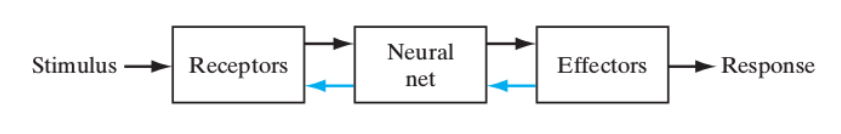
\includegraphics[width=\textwidth, scale=0.5]{Images/Ann}

 \caption[Brain Stimulus]{\textgreek{Τρόπος επικοινωνίας νευρώνων στον ανθρώπινο εγκέφαλο} \cite{brain_neuron}}
 \label{fig:stimulus}
\end{figure}

\textgreek{Ιδανικά, ένα μαθηματικό μοντέλο ενός νευρωνικού δικτύου προσομοιώνει την συμπεριφορά του βιολογικού νευρωνικού δικτύου. Για να επιτευχθεί κάτι τέτοιο, οι επιστήμονες έχουν δημιουργήσει ένα μοντέλο οποίο το οποίο αποτελείται από ένα σύνολο κόμβων οι οποίοι είναι διασυνδεδεμένοι μεταξύ τους και ανταλλάσουν πληροφορία. Ένα παράδειγμα βρίσκεται στην εικόνα }\ref{fig:ann}. \textgreek{Το θέμα των τεχνητών νευρωνικών δικτύων} (ANN) \textgreek{είναι πολύ ενδιαφέρον και συνεχίζει να είναι καθώς μας ανοίγει τον δρόμο προς την τεχνητή νοημοσύνη. Επίσης, όπως θα δούμε παρακάτω υπάρχουν πολλά είδη τέτοιων μοντέλων που έχουν πληθώρα εφαρμογών ανάλογα με το πρόβλημα.}

\begin{figure}[H]
 \centering
 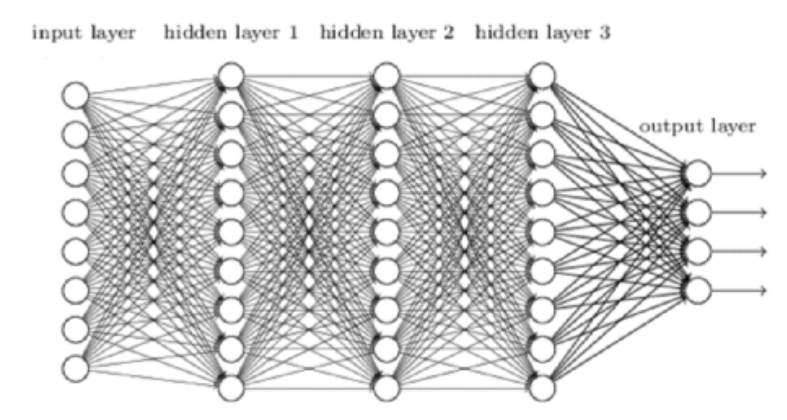
\includegraphics[width=\textwidth, scale=0.3]{Images/ann_2}

\caption[\textgreek{Νευρωνικό Δίκτυο}]{\textgreek{\textbf{Τεχνητό Νευρωνικό Δίκτυο}. Η είσοδος αποτελείται από κόμβους οι οποίοι δέχονται ένα γεγονός. Η επεξεργασία γίνεται εσωτερικά στους εσωτερικούς κόμβους. Ο αριθμός των επιπέδων ενός Δικτύου δεν είναι προκαθορισμένος και μπορεί να περάσει από πολλά επίπεδα μέχρι να πάρουμε στην έξοδο ένα επιθυμητό αποτέλεσμα.} \cite{brain_neuron}}
 \label{fig:ann}
\end{figure}

\section{\textgreek{Συνελικτικά Νευρωνικά Δίκτυα} (CNN)}
\textgreek{Μια κατηγορία Νευρωνικών Δικτύων είναι τα Συνελικτικά Νευρωνικά Δίκτυα, τα οποία έχουν εφαρμογές σε προβλήματα επεξεργασίας εικόνας και υπολογιστικής όρασης. Αποτελούνται από ένα ή περισσότερα επίπεδα συνέλιξης}
(convolutional layers) \textgreek{συχνά ακολουθούμενα από ένα επίπεδο υποδειγματοληψίας ακολουθούμενο από ένα ή περισσότερα πλήρως διασυνδεδεμένα επίπεδα όπως συναντάμε και σε ένα πολυεπίπεδο Νευρωνικό Δίκτυο. Η αρχιτεκτονική του ΣΝΔ σχεδιάζεται έτσι ώστε να εκμεταλλεύεται την δισδιάστατη δομή των εικόνων εισόδου ή άλλα δισδιάστατα σήματα όπως σήματα ήχου (π.χ. Φασματόγραμμα). Αυτό επιτυγχάνεται με τοπικές συνδέσεις και κατάλληλα βάρη προκειμένου να δημιουργηθούν χαρακτηριστικά ανεξαρτήτως μετατοπίσεων } (translation-invariant). \textgreek{Άλλο ένα πλεονέκτημα των ΣΝΔ είναι ότι είναι ευκολότερα στην εκπαίδευση και έχουν πολύ λιγότερες παραμέτρους από τα ΝΔ που έχουν πλήρως συνδεδεμένα επίπεδα.

\par 
Η είσοδος σε ένα επίπεδο συνέλιξης είναι μια $m\times n\times c$ εικόνα όπου $m$ και $n$ είναι το ύψος και το πλάτος της εικόνας αντίστοιχα, ενώ το $c$ είναι ο αριθμός των καναλιών, για παράδειγμα για έγχρωμες εικόνες }RGB $c = 3$. \textgreek{Το επίπεδο συνέλιξης έχει $k$ φίλτρα} (kernels) \textgreek{μεγέθους $w\times w \times r $ όπου είναι μικρότερο από τη διάσταση της εικόνας και μπορεί να είναι ίδιου μεγέθους με τα κανάλια ή μικρότερου και μπορεί να ποικίλει για κάθε φίλτρο. Το μέγεθος των φίλτρων προκαλεί τοπικά συνδεδεμένη δομή όπου το καθένα συνελίσσεται με κάθε εικόνα για να παράγουν χάρτες χαρακτηριστικών} (feature maps) \textgreek{μεγέθους $(m-w+1)\times (n-w+1)$. Κάθε χαρακτηριστικό υποδειγματοληπτείται τυπικά με κάποιο} pooling \textgreek{επίπεδο σε $p\times p$ συνεχείς περιοχές όπου το $p$ παίρνει συνήθως τιμές μεταξύ 2 και 5 αλλά για μεγάλες εικόνες εισόδου συναντάμε και μεγαλύτερα. Πριν ή μετά το }pooling layer \textgreek{συνήθως ακολουθεί μια προσθήκη μίας παραμέτρου πόλωσης }(bias) \textgreek{και μια συνάρτηση ενεργοποίησης σε κάθε χάρτη χαρακτηριστικών. Η εικόνα }\ref{fig:conv_layer} \textgreek{μας δείχνει ένα παράδειγμα ενός επιπέδου συνέλιξης.}

\begin{figure}[H]
 \centering
 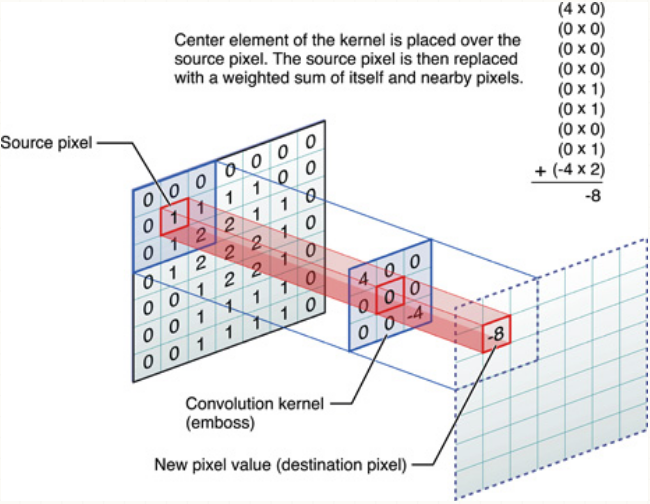
\includegraphics[width=\textwidth, scale=0.5]{Images/cnn_layer}
\caption[\textgreek{Επίπεδο Συνέλιξης}]{\textgreek{Επίδειξη ενός βήματος εφαρμογής ενός μικρού μεγέθους φίλτρου ($3\times 3$) σε έναν χάρτη χαρακτηριστικών εισόδου και το αποτέλεσμά της} \cite{cnnprimer}.}
 \label{fig:conv_layer}
\end{figure}
%%% LENET
\textgreek{Στην εικόνα }\ref{fig:lenet} \textgreek{βλέπουμε την πρώτη αρχιτεκτονική} CNN \textgreek{από τον }Yann LeCun \textgreek{για εφαρμογή σε προβλήματα αναγνώρισης ψηφίων. }

\begin{figure}[H]
 \centering
 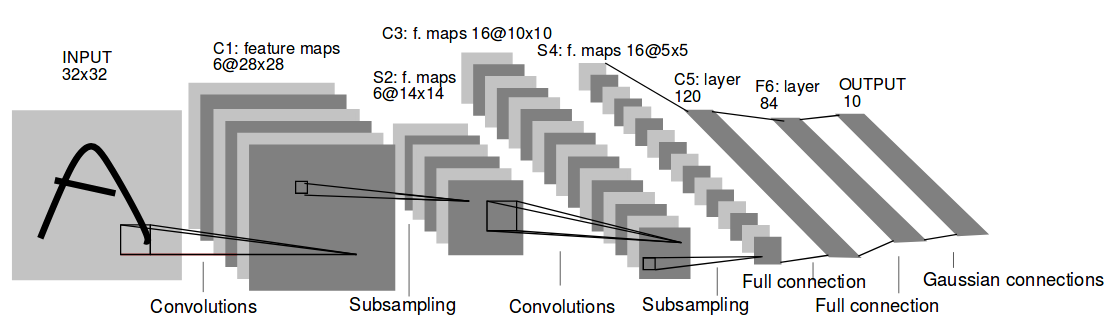
\includegraphics[width=\textwidth, scale=0.5]{Images/lenet_5}
\caption[\textgreek{ΣΝΔ }Lenet-5]{\textbf{CNN LeNet-5}.\textgreek{Αρχιτεκτονική του πρώτου Συνελικτικού Νευρωνικού Δικτύου για αναγνώριση ψηφίων από εικόνες. Κάθε επίπεδο αποτελεί ένα χαρτογράφημα των χαρακτηριστικών} \cite{lecun_net}.}
 \label{fig:lenet}
\end{figure}

\textgreek{Το } Alex-Net \textgreek{(εικόνα \ref{fig:alexnet_img}) ήταν μια δημιουργία των }Alex Krizhevsky, Ilya Sutskever, \textgreek{και} Geoffrey Hinton, \textgreek{και σηματοδότησε μια νέα εποχή στην υπολογιστική όραση καθώς πλέον περάσαμε στα \emph{Βαθιά} ΝΔ. Το εφάρμοσαν σε ένα από τα πιο απαιτητικά προβλήματα, το} \href{http://www.image-net.org/}{\emph{Image-Net}} \cite{imagenet_bib}. \textgreek{Η συγκεκριμένη αρχιτεκτονική κατάφερε να πετύχει ένα σημαντικό αποτέλεσμα μειώνοντας πάνω από 10\% το σφάλμα σε σχέση με τον προηγούμενο νικητή το 2012, πάνω σε ένα πρόβλημα με 15 εκατομμύρια εικόνες και 1000 κατηγορίες για αναγνώριση. Σε αυτό το μοντέλο ήταν και η πρώτη εφαρμογή των γραμμικών ανορθωτών ως συνάρτηση ενεργοποίησης αλλά και η χρήση συνθετικών δεδομένων. Αυτή η συνεισφορά είναι τόσο σημαντική καθώς οι περισσότερες τεχνικές χρησιμοποιούνται μέχρι και σήμερα.}

%% ALEXNET
\begin{figure}[H]
 \centering
 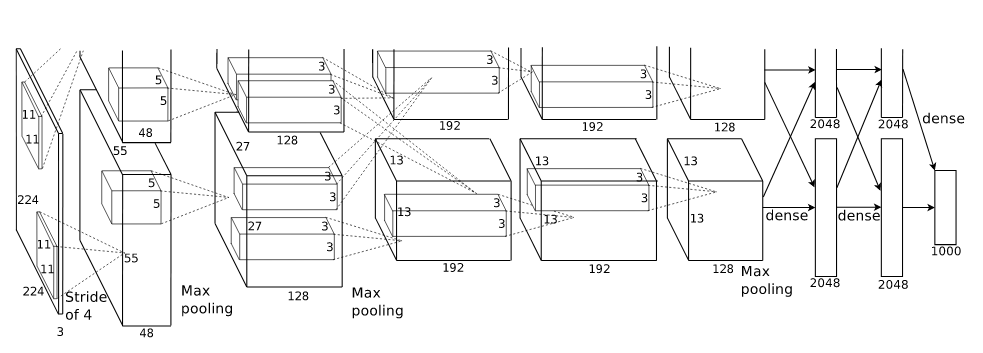
\includegraphics[width=\textwidth, scale=0.5]{Images/alex_net}
\caption[\textgreek{ΣΝΔ }Alex-Net]{\textbf{Alex-Net}.\textgreek{Αρχιτεκτονική του }Alex-Net \textgreek{ένα από τα πρώτα Βαθιά ΝΔ με 60 εκατομμύρια παραμέτρους και 650.000 νευρώνες.} \cite{alex_net_bib}.}
 \label{fig:alexnet_img}
\end{figure}

\section{\textgreek{Πλήρως Συνελικτικά Νευρωνικά Δίκτυα}}
\textgreek{Μία ακόμα κατηγορία ΝΔ με τα οποία θα ασχοληθούμε στο υπόλοιπο της εργασίας είναι τα Πλήρως ΣΝΔ} (Fully-CNN) \cite{fcnn_1}. \textgreek{Η κύρια διαφορά με τα ΣΝΔ είναι η απώλεια πλήρως συνδεδεμένων επιπέδων στην έξοδο }(fully-connected layers), \textgreek{εν αντιθέσει με τα ΣΝΔ που είδαμε προηγουμένως, δηλαδή τα ΠΣΝΔ μαθαίνουν πληροφορία μόνο από φίλτρα. Τα ΠΣΝΔ θεωρούνται κατάλληλα για προβλήματα Σημασιολογικής Κατάτμησης αντικειμένων από εικόνες (εικόνα} \ref{fig:fcn_img}).

%FCN_1
\begin{figure}[H]
 \centering
 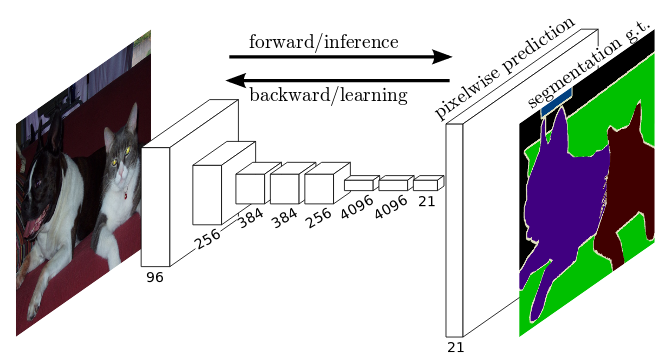
\includegraphics[width=\textwidth, scale=0.5]{Images/fcn_1}
\caption[Fully-CNN]{\textgreek{Πλήρως ΣΝΔ} (Fully CNN) \textgreek{μπορούν να μάθουν αποδοτικά να κάνουν προβλέψεις σε προβλήματα αναγνώρισης σε επίπεδο εικονοστοιχείων} \cite{fcnn_1}.}
 \label{fig:fcn_img}
\end{figure}



\textgreek{Μερικά θετικά στοιχεία που καταστούν τα ΠΣΝΔ κατάλληλα για Σημασιολογική Κατάτμηση είναι σε αντίθεση με άλλου είδους ΝΔ είναι}:

\begin{description}[labelindent=10pt, style=multiline, leftmargin=30pt]
 \item[1.] \textgreek{Χρησιμοποιούν όλη την πληροφορία της εικόνας.}
 \item[2.] \textgreek{Κρατάνε την χωρική πληροφορία} (spatial information) \textgreek{από την εικόνα.}
 \item[3.] \textgreek{Είναι πιο γρήγορα στην εκπαίδευση αλλά και στην συμπερασματολογία.}
 \item[4.] \textgreek{Είναι αμετάβλητα ως προς το μέγεθος εισόδου της εικόνας.}
\end{description}
\pagebreak
\section{\textgreek{Εμπρόσθια Διάδοση}}
\textgreek{Η Εμπρόσθια Διάδοση }(Forward Propagation) \textgreek{είναι ο τρόπος με τον οποίο το ΣΝΔ επεξεργάζεται τα δεδομένα. Τα ΣΝΔ έχουν δημιουργηθεί με την προοπτική να επεξεργάζονται δεδομένα από εικόνες. Αποτελούνται από πολλά επίπεδα συνέλιξης τα οποία είναι συνδεδεμένα σειριακά για να επεξεργάζονται οπτική πληροφορία. Τα συνελικτικά επίπεδα αποτελούνται από μια σειρά από φίλτρα $\mathbf{\mathit{K}}$ και τις πολώσεις $\mathbf{\mathit{b}}$} (biases), \textgreek{ ενώ δέχονται έναν χάρτη χαρακτηριστικών στην είσοδο $\mathbf{\mathit{I}}$.}
\par
\textgreek{Στην περίπτωση που έχουμε εικόνες για αναγνώριση, η είσοδος αποτελείται από μια εικόνα με ύψος $\mathbf{\mathit{H}}$, πλάτος $\mathbf{\mathit{W}}$  και αριθμό καναλιών $\mathbf{\mathit{C =3 }}$ (κόκκινο, πράσινο και μπλε), $\mathbf{\mathit{I \in \mathbb{R}^{H\times W\times C}}}$. Επομένως, για μια σειρά από $D$ φίλτρα έχουμε $K \in \mathbb{R}^{k_1\times k_2\times C\times D}$ και $b \in \mathbb{R}^{D}$ πολώσεις, μία για κάθε φίλτρο. Για κάθε στοιχείο $i,j$ του χάρτη χαρακτηριστικών εισόδου $I$ εφαρμόζουμε την συνέλιξη με τον πυρήνα $K$:}

\begin{equation}
(I \ast K)_{ij} = \sum_{m=0}^{k_1-1} \sum_{n=0}^{k_2-1} \mathit{K_{m,n,c}} \cdot \mathit{I_{i+m,j+n,c}} + \mathit{b}
\end{equation}

\textgreek{Πιο αναλυτικά, η παραπάνω εξίσωση αναλύεται για κάθε επίπεδο συνέλιξης με τις εξής παραμέτρους:}

\begin{enumerate}
 \item l : \textgreek{Συμβολίζει το επίπεδο συνέλιξης $l$ όπου $l = 1$ είναι το πρώτο επίπεδο και $l = L$ το τελευταίο επίπεδο.}
\item \textgreek{$x$ είναι η είσοδος με διαστάσεις $H\times W$ και με $i,j$ συμβολίζουμε τους δείκτες του πολυδιάστατου διανύσματος.}
\item \textgreek{Φίλτρο $w$ διαστάσεων $k_1\times k_2$ όπου έχει ως δείκτες τα $m,n$.}
\item \textgreek{$w_{m,n}^{l}$ είναι ο πίνακας με τα βάρη που συνδέει του νευρώνες του επιπέδου $l$ με τους νευρώνες του επιπέδου $l-1$.}
\item \textgreek{$x_{i,j}^{l}$ είναι το διάνυσμα εισόδου του επιπέδου $l$}:\\[1em]
\centerline{ $x_{i,j}^{l} = \sum_{m} \sum_{n} w_{m,n}^{l} o_{i+m,j+n}^{l-1} + b^{l}$}

\item \textgreek{$b^{l}$ είναι το διάνυσμα πόλωσης.}
\item \textgreek{$o_{i,j}^{l}$ είναι το διάνυσμα εξόδου στο επίπεδο $l$}:\\[1em]
\centerline{$ o_{i,j}^{l} = f(x_{i,j}^{l})$}
\item \textgreek{ $f(\cdot)$ είναι η συνάρτηση ενεργοποίησης, η οποία εφαρμόζεται στην είσοδο μετά την διαδικασία της συνέλιξης στο επίπεδο $l$.}
\end{enumerate}

\pagebreak
\section{\textgreek{Αλγόριθμος Οπισθοδρόμησης}}
\textgreek{Ο αλγόριθμος οπισθοδρόμησης }(backpropagation) \cite{bptt_1} \textgreek{αποτελεί την μέθοδο με την οποία ένα ΝΔ επαναπροσδιορίζει τις παραμέτρους του. Αποτελεί έναν από τους πιο βασικούς αλγορίθμους για την εκπαίδευση των ΝΔ σε προβλήματα επιβλεπόμενης μάθησης }(supervised learning). \textgreek{Η συνάρτηση κόστους που χρησιμοποιούμε σε αυτό το πρόβλημα όπως θα αναλύσουμε παρακάτω (παράγραφος }\ref{sec:loss_function})\textgreek{ είναι η συνάρτηση διεντροπίας και είναι παραγωγίσιμη και έχει πολύ απλή παράγωγο.}
\par
\textgreek{Ο αλγόριθμος οπισθοδρόμησης χρησιμοποιείται για τον υπολογισμό των παραγώγων σφάλματος. Ο αλγόριθμος αποτελείται από την εφαρμογή του κανόνα της αλυσίδας για τον υπολογισμό των μερικών παραγώγων. Αρχικά, υπολογίζουμε την μερική παράγωγο της συνάρτησης κόστους ως προς την μεταβλητή εξόδου και την μερική παράγωγο της εξόδου από την } softmax ($y_i$) \textgreek{ως προς την μεταβλητή της εισόδου της μονάδας }softmax ($s_i$). \textgreek{Επομένως, χρησιμοποιώντας τον κανόνα της αλυσίδας για να υπολογίσουμε τις παραγώγους της συνάρτησης κόστους ως προς την είσοδο της μονάδας }softmax. \textgreek{Στις εξισώσεις παρακάτω, $y_i$ είναι η έξοδος του $i$ στοιχείου ενώ $s_i$ είναι η η είσοδος του $i$ στοιχείου }\cite{backprop_notes}.  

\begin{equation}
 \frac{\partial E}{\partial y_i} = -\frac{t_i}{y_i}
\end{equation}

\begin{equation}
 \frac{\partial y_i}{\partial s_i} = y_i(1-y_i)
\end{equation}

\begin{equation}
 \frac{\partial E}{\partial s_i} =\frac{\partial E}{\partial y_i} \frac{\partial y_i}{\partial s_i} = y_i-t_i
\end{equation}
\textgreek{Εφαρμόζοντας τον κανόνα της αλυσίδας, προχωράμε προς τα κρυφά επίπεδα }(hidden layers) \textgreek{προς τα πίσω. Για να διαδώσουμε τις παραγώγους του $i$ στοιχείου στο $j$ στοιχείο το οποίο ανήκει στο προηγούμενο επίπεδο, προκύπτουν οι παρακάτω εξισώσεις} (\ref{eqn:back_4} \textgreek{και} \ref{eqn:back_5}) \textgreek{όπου $w_{ji}$ είναι το βάρος που ανατίθεται στην σύνδεση μεταξύ της εισόδου του $j$ στοιχείου με την κρυφή μονάδα $i$. Εφαρμόζοντας επαναληπτικά τον κανόνα της αλυσίδας διαδίδουμε τις παραγώγους του σφάλματος προς την είσοδο του ΝΔ. Με αυτήν την μέθοδο έχουμε καταφέρει να υπολογίσουμε τις παραγώγους σφάλματος για κάθε βάρος.}

\begin{equation}
\label{eqn:back_4}
 \frac{\partial E}{\partial y_i} =\frac{\partial E}{\partial s_i} \frac{\partial s_i}{\partial y_j}=\sum_i w_{ji} \frac{\partial E}{\partial s_i} 
\end{equation}

\begin{equation}
\label{eqn:back_5}
\frac{\partial E}{\partial w_{ji}} =\frac{\partial E}{\partial s_i} \frac{\partial s_i}{\partial w_{ji}} = (y_i-t_i)\frac{\partial s_i}{\partial w_{ji}}
\end{equation}

\textgreek{Στα επίπεδα συγκέντρωσης διαφέρει η διαδικασία της οπισθοδρόμησης ανάλογα με το είδος του επιπέδου συγκέντρωσης. Ένα επίπεδο συγκέντρωσης δεν περιέχει παραμέτρους μάθησης} \cite{pooling}.\textgreek{ Τα πιο δημοφιλή επίπεδα συγκέντρωσης είναι τα επίπεδα μέγιστης και μέσης συγκέντρωσης αντίστοιχα. Στο επίπεδο συγκέντρωσης, η εμπρόσθια διάδοση έχει ως αποτέλεσμα στην έξοδο έναν μειωμένο χάρτη χαρακτηριστικών όπου έχει εφαρμοστεί ένα $N\times N$ τμήμα συγκέντρωσης σε κάθε περιοχή και στην έξοδο εξέρχεται μόνο ένα στοιχείο από το τμήμα. Η Οπισθοδρόμηση στο επίπεδο συγκέντρωσης, οπισθοδρομεί το σφάλμα το οποίο έχει προέλθει από την μοναδική επικρατέστερη τιμή του κάθε τμήματος. 
\par 
Για να κρατήσουμε την θέση της επικρατέστερης τιμής από το επίπεδο συγκέντρωσης, σημειώνουμε την θέση κατά την εμπρόσθια διάδοση και μετά την χρησιμοποιούμε για να οδηγήσουμε τις παραγώγους του σφάλματος κατά την οπισθοδρόμηση. Η δρομολόγηση των παραγώγων επιτυγχάνεται με κάποια από τις παρακάτω μεθόδους, ανάλογα το επίπεδο συγκέντρωσης}:
\par 
% 
\begin{description}[labelindent=1.7cm, style=unboxed, leftmargin=2.1cm, font=$\bullet$~]
  \item[Max-Pooling] \textgreek{Το σφάλμα απλώς ανατίθεται στο στοιχείο το οποίο επικράτησε κατά το εμπρόσθιο πέρασμα. }
  \item[Average-Pooling] \textgreek{Το σφάλμα πολλαπλασιάζεται με τον παράγοντα $\frac{1}{N\times N}$ και η προκύπτουσα τιμή ανατίθεται σε ολόκληρο το τμήμα συγκέντρωσης, δηλαδή όλα τα στοιχεία παίρνουν την ίδια κανονικοποιημένη τιμή.} 
\end{description}


